\subsection{Motivation and Theory}

\begin{frame}
	\frametitle{1) Motivation and Theory}
	\textbf{Q: Why are semiconductors interesting?}
	
	Applications.\footnote{\tiny{W. Demtröder. \textit{Experimentalphysik 3: Atome, Moleküle und Festkörper}. 5. Auflage. Springer, Berlin, 2016.}}\footnote{\tiny{Semiconductors.org. \url{https://www.semiconductors.org/}. Accessed on the 15.11.2021.}}
	\begin{itemize}
	    \item Energy conversion: e. g. photovoltaic
	    \item Computer industry: e. g. 'Silicon Valley'
	\end{itemize}
	\begin{figure}[H]
  		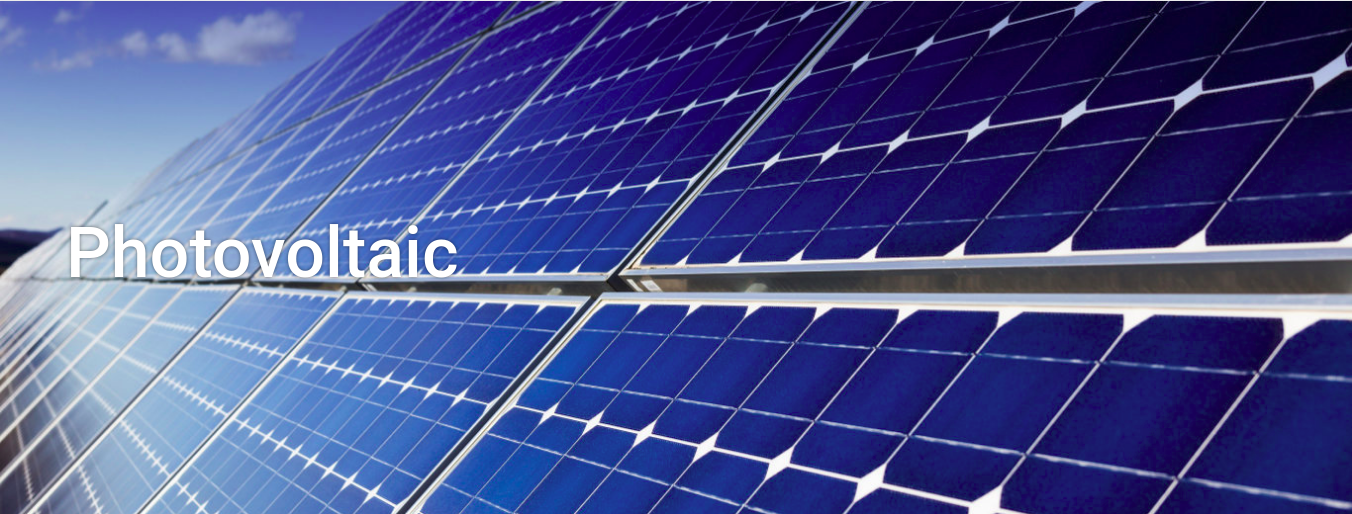
\includegraphics[width=0.6\textwidth]{images/chapter1/1_photovoltaic.png} 
  		\caption*{ales.airliquide. \url{https://ales.airliquide.com/our-markets/photovoltaic}. Accessed on the 15.11.2021.}
	\end{figure}
\end{frame}


